\subsection{Hardware}

Unabhängig von der Zusammenstellung umfänglicher Speicherlösungen, müssen die Daten trotzdem irgendwann auf einen Hardwarespeicher geschrieben werden. Folgender Abschnitt erläutert, die allgemeine Funktion und geht auf einige der häufigsten verwendeten Typen ein.

\subsubsection{Hard Disk Drive (HDD)}

Hierbei handelt es sich um einen nicht volatilen Speicher, der digital kodierten Inhalte auf der magnetischen Oberfläche einer Platte speichert. Traditionell gibt es zwei Protokolle: SAS im kommerziellen Sektor und SATA im privaten \parencite{wikibooks.2016}.

Ein oder mehrere Leseköpfe werden mithilfe von Armen und einem Servomotor über die Platte bewegt, um relevante Stellen auszulesen. Bei der Herstellung von HDDs werden Tracks in die Platte geschrieben, die jeweils ein Label und Blockinformationen besitzen. Durch sie ist es einfacher den Lesekopf zu platzieren. Jeder dieser Tracks kann bis zu einigen MBs an Daten beinhalten. Durch die Blockbildung bei I/O Operationen kann häufig nur ein einzelner Block (64-256) Block geschrieben werden, wodurch Festplatten unnötig langsam werden. Durch neue Technologie können IOs gequeued, sodass die Platte kontinuierlich lesen und schreiben kann. Trotzdem ist nur eine maximale Geschwindigkeit von ungefähr 300 \gls{IOPS} das Limit für Platten mit 10.000 RPM \parencite[Kap. 3]{kaufmann.2016}.

Jede Festplatte hat heutzutage einige private Sektoren, auf denen Reparatur Informationen und Reserveblöcke gespeichert sind. Fällt ein Block in der Festplatte aus (durch zum Beispiel physikalische Beschädigung), kann dieser fließend ersetzt werden, sodass keine Daten verloren gehen. Kurz vor dem Ausfall einer Platte steigt diese Anzahl der Lesefehler einer Platte massiv an, sodass eine Datenreovery versucht werden kann. Leider ist dies keine verlässliche Methode, um Daten zu sichern, sodass andere Methoden verwendet werden sollten \parencite[Kap. 3]{kaufmann.2016}.

Um Datenverlust durch Plattenausfälle entgegenzuwirken, besteht die Möglichkeit der Verwendung von so genannten RAIDs. Dies ist eine Methode, bei der mehrere HDDs so zusammengeschaltet werden, sodass bei dem Ausfall einer Einzelner die Daten weiterhin verfügbar sind \parencite{wikibooks.2016}.

Festplatten sind gut erforscht, es treten extrem selten unbekannte Probleme auf und werden seit Jahrzehnten verwendet, ihr Speicher ist extrem günstig geworden und in Masse verfügbar. Ihr größter Nachteil ist eine sehr geringe I/O Geschwindigkeit im Vergleich mit neueren Technologien \parencite[Kap. 3]{kaufmann.2016}.

\subsubsection{Solid State Drive (SSD)}

In 2007 wurde der erste SSD Speicher vermarktet und stach durch extrem hohe Zugriffszahlen heraus. Diese sind waren bei 4000 \gls{IOPS} bereits um das zehnfache höher als die klassischer Festplatten. Heutzutage ist es möglich IOPS Zahlen im Millionenbereich zu erreichen, was eine Revolution für Speicher bedeutet \parencite[Kap. 3]{kaufmann.2016}.

\begin{figure}[hbt]
	\centering
	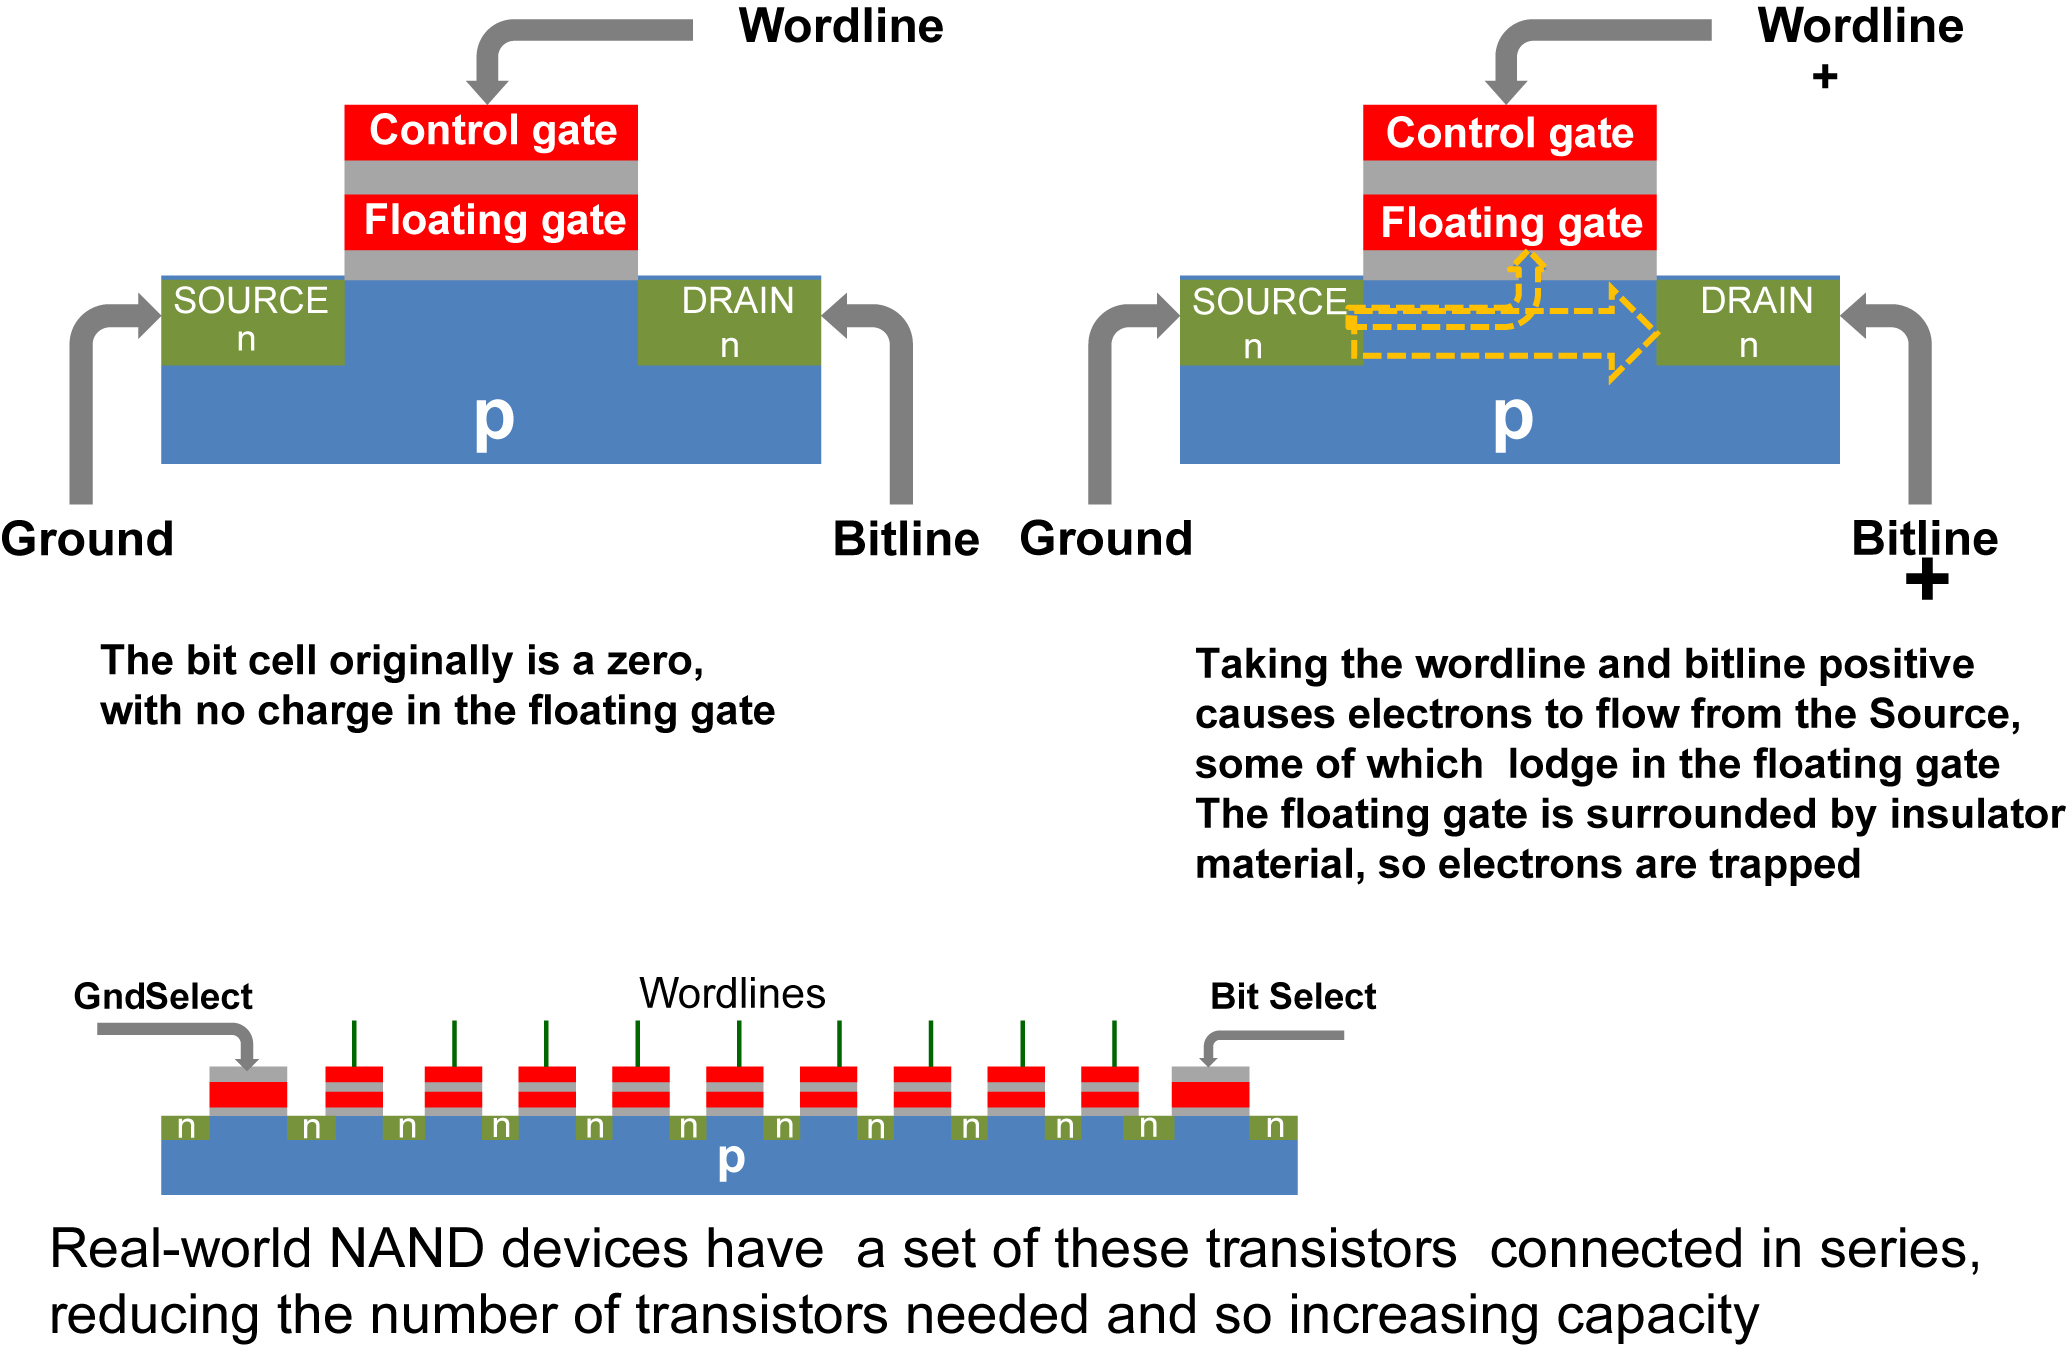
\includegraphics[scale=0.85]{images/flash}
	\caption{Funktionsweise eines NAND Flash Speichers \parencite{kaufmann.2016}}
	\label{fig:flash}
\end{figure}

SSDs benutzen Nicht-Und (NAND) memory chips zum Speichern einzelner Bitinformationen. Von diesen Zellen gibt es dann einige Millionen, die beliebig adressiert werden können (Random Access Memory). Innerhalb eines so genannten Floating Gate können nun Elektronen eingefangen werden, um eine binäre Eins zu repräsentieren. Im Ausgangszustand sind diese ``Fallen'' leer, um einen Nullinformationen zu speichern. Sobald der Speichercontroller eine Zellen laden will, wird der Einlasstransistor geöffnet und einige Elektronen in der Zelle für eine beliebig lange Zeit gefangen.

Dieser Prozess findet in \autoref{fig:flash} statt, wenn auf der Bit- und Wordline eine positive Ladung gesetzt wird. Meistens liegen mehrere Zellen auf einer Reihe, was den Lese Prozess verkomplizieren kann. Es wird eine niedrige Spannung an alle Wordlines angelegt, wodurch bei geladenen Zellen eine Konduktivität festgestellt werden kann. 

Wird eine einzelne Zelle zu häufig beschrieben, kann diese Isolation verlieren, wodurch sie unnutzbar zum Speichern wird. Schreibstrategien und Reservezellen werden verwendet, um dies vorzubeugen.	

Zum Löschen der Zellen wird eine hohe negativer Spannung an die Zellen angelegt, wodurch die gefangenen Elektronen aus den Floating Gates heraus gedrückt werden. Dies passiert meistens in fest definierten Pages, sodass keine speziellen Blöcke gelöscht werden können. Nach dem Löschen eines Blockes wird dessen Zeiger auf eine vorher geleerte Page bewegt und der Block als ``discared'' markiert. Sind innerhalb einer Page genug Blöcke in diesem Zustand, werden die verbleibenden Daten verschoben und die gesamte Page gelöscht und Teil des freien Speichers der SSD \parencite{kaufmann.2016}. 
Durch diesen Prozess ist das Löschen von Dateien nicht mehr zuverlässig, da die Daten noch für lange Zeit innerhalb eines ``discared'' Blockes liegen können, der erst wesentlich später, vom Controller gelöscht wird.

SSDs können über das SATA Protokoll angeschlossen werden, aber in den letzen Jahren wurde das wesentlich performantere NVMe entwickelt.

Da dieser Speicher keine sich bewegende Teile hat, ist er wesentlich robuster was Schläge, Vibrationen und hohe Temperaturen angeht. Ebenfalls ist der Strombedarf wesentlich geringer, was zusammen mit den vorherigen Punkten den Betrieb von SSDs in großen Rechenzentren wesentlich einfacher und günstiger macht.

Trotzdem gibt es auch einige Nachteile von Flashspeicher: Die meisten Anwendungen sind nicht darauf ausgelegt, so hohe Zugriffszahlen zu unterstützen. In der Vergangenheit hat I/O immer ein Bottleneck in Applikationen dargestellt, sodass die meisten Programme entsprechenden designed wurden.
Diese zieht sich durch die gesamte Softwarelandschaft und auch die geläufigen Betriebssysteme sind nicht in der Lage diese neue Geschwindigkeit voll auszunutzen. Ebenfalls ist das SATA Interface nicht perfekt für SSDs, da es ursprünglich dafür designed war, die niedrigen Bandbreiten von Festplatten auszugleichen \parencite[Kap. 3]{kaufmann.2016}.


\subsubsection{Bandlaufwerk}

Bandlaufwerke funktionieren im Grund wie die früher verwendeten Kassetten. Innerhalb des Laufwerkes befindet sich ein dünner Streifen aus Plastik mit einer magnetischen Oberfläche. Dieser wird, ähnlich wie bei Festplatten, mit digitalen Daten beschrieben. 

Es kann nicht auf beliebige Bereich des Bandes zugegriffen werden, Lesen und Schreiben erfolgt immer sequentiell. Das Laufwerk muss von Anfang bis Ende durchlaufen werden, um I/O Aktionen durchführen zu können \parencite{adrc.2009}.

Ein Bandlaufwerk verwendet einen kleinen Motor, um das Band auf- und abzuwickeln. Dabei wandert dieses entlang eines Lese- und Schreibkopfes. Um Unterschiede zwischen der Geschwindigkeit der ankommenden Daten vom Computer und der begrenzten \gls{IOPS} des Laufwerkes auszugleichen, wird eine Steuereinheit verwendet. Diese regelt Fehlerhandling, Puffer und andere logische Operationen.

Informationen werden in die Steuereinheit geladen und dann auf das Band geschrieben. Dieser Prozess wiederholt sich solange bis keine Daten mehr vorhanden sind.

Aufgrund von geringen Kosten und hoher Lebenszeit wird diese Art von Laufwerk immer noch häufig verwendet. Besonders of wird es für Backup Szenarien genutzt, da hier die Nachteile des nur sequentiellen Zugriffes auf Daten keine große Rolle spielt \parencite{adrc.2009}. 

\subsection{Speicher Anbindung über Netzwerke}
\subsubsection{Direct Attached Storage (DAS)}

Bei Direct Attached Storage handelt es sich um externen Speicher, der direkt mit einem oder mehreren Servern über ein SCSI Interface verbunden ist. Dabei wird kein Netzwerk verwendet. Es gibt verschiedene Typen von DAS, bei manchen werden nur beliebige Platten zusammengewürfelt (\ac{JBOD}), bei anderen ganze Plattenarrays angeschlossen.
Hierbei handelt sich um den ältesten Speichertypen, der lange vor dem Entstehen von SAN oder NAS verwendet wurde.

Es kann nur eine begrenzte Anzahl von DAS an einen Rechner angeschlossen werden, da die Anzahl von SCSI Schnittstellen an Servern limitiert ist. Dadurch ist diese Art von Speicher leider nur begrenzt skalierbar.

Ein weiterer großer Nachteil von direkt angebunden Speicher ist, dass bei einem Ausfall des Servers ein wesentlicher Teil der Daten nicht mehr erreichbar ist. Die Verfügbarkeit der Daten hängt also nicht nur vom Speicher selber ab, sondern auch von dem bereitstellenden Server.

Wird das Laufwerk an mehrere Server angeschlossen, um obigen Problem entgegen zu wirken, erhöht sich durch einen Ausfall die Zugriffszeit beträchtlich \parencite[Kap. 1, Disk Storage Systems]{gupta.2002}.

Der größte Vorteil von DAS Geräten ist, dass sie einfach aufzusetzen und zu warten sind, da keine Netzwerkkenntnisse oder Hardware benötigt wird. Dies bedeutet geringe Kosten und einfache Handhabung \parencite{beal.2017}.

\subsubsection{Network Attached Storage (NAS)}

Network Attached Storage stellt ein einfaches System dar, um Daten an einer einheitlichen Stelle im Netzwerk zu speichern. Hierdurch werden die Daten von den Servern selber wegbewegt zu speziell zur Speicherung ausgelegten Hardware. 

Ein NAS Gerät ist spezialisierte Hardware mit meist zugehöriger Management Software. In den meisten Fällen muss es nur mit dem Firmen Netzwerk verbunden und eingeschaltet werden. Ebenfalls ist der Speicher plattformunabhängig und kann mithilfe verschiedener Protokolle von jedem Client verwendet werden. Einige Beispiele für diese sind: HTTP (Internetanfragen), FTP oder TCP/IP. Ebenfalls können Datenanfragen über NFS (für Linux)oder SMB (für Windows) getätigt werden \parencite[Kap. 1, NAS Devices]{gupta.2002}.

Bei einem Daten Request wird die Anfrage an das NAS Gerät weitergeleitet, das die notwendige Daten an dem Server zurück sendet, welcher diese dem Client zur Verfügung stellt.

NAS besitzt einige Vorteile: Es gibt eine deutliche Performance Steigerung bei den Anwendungsservern, da I/O Operationen komplett auf der dedizierten Hardware ausgeführt werden. NAS Devices besitzen eine wesentliche bessere Skalierbarkeit als DAS Geräte, es können beliebig viele neue Netzwerkspeicher zu einem System hinzugefügt werden.

Ebenfalls ist die Fehleranfälligkeit wesentlich geringer, wenn ein Anwendungsserver abstürzt, bleibt der Zugriff auf den NAS im Netzwerk immer noch erhalten.

Management und Einsatz sind auch einfach gehalten, die Geräte konfigurieren sich zu großen Teilen selber und sind mit jedem System ansprechbar.

Trotz all dieser Vorteile gibt es, besonders in großen Netzwerken, auch einige Nachteile. Anfragen von Clients erzeugen eine große Menge Netzwerk Verkehr, die viel Bandbreite beansprucht. Sobald viele Request gleichzeitig auftreten, kann es deswegen auch zu Performance Einbrüchen kommen.

Durch die Zentralisierung des Speichers wird dieser auch einfacher anfällig für bösartige Attacken, Netzwerk Verkehr kann abgefangen oder modifiziert werden \parencite[Kap. 1, Adv. and Disadv. of NAS Devices]{gupta.2002}.


\subsubsection{Storage Area Network (SAN)}
SAN wurden entwickelt, um enorme Mengen von Daten zu verarbeiten. Sie werden nicht direkt in das Client oder Server Netzwerk eingebunden, sondern bilden eine eigenes, das die verschiedenen Speicher miteinander verbindet. Dieses kann dann nur durch die SAN Server angesprochen werden. Dies führt zu einem sehr sicheren Setup, da die Geräte von den Clients komplett verborgen sind \parencite[Kap. 1, SANs]{gupta.2002}.

Es gibt mehrere wichtige Bestandteile: Die oben erwähnten Server stellen den Zugriffspunkt für Applikationsserver im normalen Netzwerk. Innerhalb des Netzwerks kann es verschiedene Speichertypen geben (RAIDs, JOBDs, Disk Storage Systems, Bandlaufwerke).
Interfaces werden verwendet, um den Speicher zu den Server zu verbinden uns sie damit zu externalisieren. Mithilfe von SAN Interconnects können entfernte Speicher ebenfalls eingebunden werden. Hubs und Router werden benutzt, um verschiedene Speicher zusammenzuschließen, wobei Router das Signal immer nur zu einem Gerät weiterleiten und es nicht broadcasten.
Außerdem gibt es noch eine ganze Reihe an weiteren Geräte, die für die Kommunikation zwischen verschiedenen Protokollen und Technologien verantwortlich sind \parencite[Kap. 2, SAN Components and Building Blocks]{gupta.2002}.

Ein vereinfachtes Setup kann in \autoref{fig:storageareanetwork} betrachtet werden.

\begin{figure}[hbt]
	\centering
	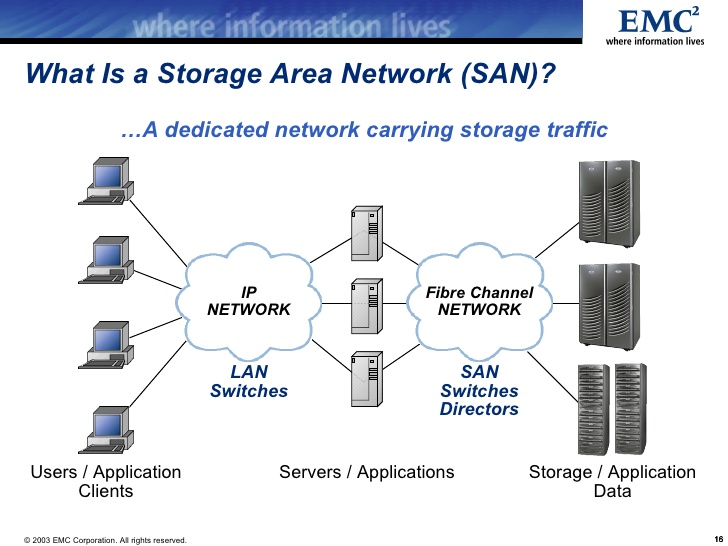
\includegraphics[scale=0.9]{images/storage-area-network}
	\caption{Typisches SAN Konstruktion \parencite[Kap. 1]{gupta.2002}}
	\label{fig:storageareanetwork}
\end{figure}

Durch dieses eigene Netzwerke können einige Vorteile ausgenutzt werden, die so bei NAS nicht oder nur schwer zu erreichen sind. Zur Verbindung der Geräte können Hochleistungsnetzwerke wie FibreChannel verwendet werden, die wesentlich performanter sind als Ethernet. Da das SAN getrennt vom Netzwerk der Applikationsserver ist, muss keine Bandbreite geteilt werden, was ebenfalls die Anwendungen schneller macht. Genauso wie bei NAS werden I/O Aktionen auf die SAN Geräte verlagert und es können zusätzlich performance intensive Backups isoliert im SAN erledigt werden \parencite[Kap. 1, SANs]{gupta.2002}.

Das Filesystem von SANs wird nicht von den Geräten selber verwaltet, sondern von den entsprechenden Fileservern. SANs bieten einfachen Blockzugriff auf die Daten, für die Server sind sie nur weitere Festplatten. Dadurch ist es einfacher das SAN beliebig zu skalieren, da einfach nur neue Speicher Geräte hinzugefügt werden müssen. Die Ausfallsicherheit wird ebenfalls höher, da meistens verschiedene Server Zugriff auf das SAN haben und einfach ein weiterer angesprochen werden kann, falls ein Ausfall stattfindet.

Es gibt optimierte Software zur Verwaltung von SANs, die höhere Performance ermöglichen.

Ein großer Nachteil von SANs ist, dass sie sehr komplex aufzusetzen sind und auch die Kosten wesentlich höher sind als bei NAS Lösungen \parencite[Kap. 2]{gupta.2002}.





